\begin{center}
  \textbf{Отчёт лабораторной работы №\envReportLabNumber}
\end{center}

\textbf{Тема}:
<<\envReportTitle>>

\textbf{Цель}: ...

% = = = = = = = = = = = = = = = =

\begin{center}
  \textbf{Задание}
\end{center}

\textbf{Условие}:
Найти графическим способом максимальное и минимальное значение целевой функции

\begin{center}
  \textbf{Вариант 5}
\end{center}

$$
\mathbb{Z} = -2 x +2 y
$$

$$
\begin{cases}
  4x - 3 y  \leq 12\\
  x + y \leq 10 \\
  2 x + y \geq 6\\
  x \geq 0, y \geq 0
\end{cases}
$$

\textbf{Решение}:

Решать буду по ролику на YouTube \cite{Youtube}.

\subparagraph{1}
Построим область допустимых значений.
Сразу начертим систему координат.
В задаче будут приниматься переменные x и y.

\subparagraph{1.1}
Начнём с первой линии.
Если неравенство ($4x - 3 y  \leq 12$) заменить знаком равно, то это будет уравнение прямой ($4x - 3 y  = 12$).
Прямую можно построить по двум точкам.
Для простоты x примем за 0, потом y.

$
\text{if } x = 0 \implies 4 \cdot 0 - 3 y = 12, -3y = 12, y=-4
$

$
\text{if } y = 0 \implies 4 x - 3 \cdot 0 = 12, 4x=12, x=3
$

Отметим точку (0; -4) и (0; 2) на графике.
Соединим точки прямой линией.
Теперь вспомним, что выражению ($4x - 3 y  \leq 12$) соответствует знак меньше или равно
- и определим какой из областей под ней или над ней нужно заштриховать.
Для простоты возьмем начало координат: точку O(0; 0)
и посмотрим удовлетворяет ли она неравенству ($4x - 3 y  \leq 12$).

$
4 \cdot 0 - 3 \cdot 0  \leq 12, 0 \leq 12 \implies \text{верно} \implies \text{O(0; 0)} \in (4x-3y\leq 12)
$

Значит точка O(0; 0) принадлежит области, значит заштрихована будет та область, в которой лежит точка O(0; 0).

Результат смотри на рисунке~\ref{fig:1}.

% = = = = =

\subparagraph{1.2}
Теперь тоже самое проделаем и со вторым условием ($x+y \leq 10$)
Если неравенство ($x+y \leq 10$) заменить знаком равно, то это будет уравнение прямой ($x+y = 10$).
Прямую можно построить по двум точкам.
Для простоты x примем за 0, потом y.

$
\text{if } x = 0 \implies 0+y=10, y=10
$

$
\text{if } y = 0 \implies x+0=10, x=10
$

Отметим точку (0; 19) и (10; 0) на графике.
Соединим точки прямой линией.
Теперь вспомним, что выражению ($x+y \leq 10$) соответствует знак меньше или равно
- и определим какой из областей под ней или над ней нужно заштриховать.
Для простоты возьмем начало координат: точку O(0; 0)
и посмотрим удовлетворяет ли она неравенству ($x+y \leq 10$).

$
0+0 \leq 10, 0 \leq 10 \implies \text{верно} \implies \text{O(0; 0)} \in (x+y\leq 10)
$

Значит точка O(0; 0) принадлежит области, значит заштрихована будет та область, в которой лежит точка O(0; 0).

Результат смотри на рисунке~\ref{fig:2}.

\subparagraph{1.3}
Теперь тоже самое проделаем и с третьим условием ($2x+y \geq 6$)
Если неравенство ($2x+y \geq 6$) заменить знаком равно, то это будет уравнение прямой ($2x+y = 6$).
Прямую можно построить по двум точкам.
Для простоты x примем за 0, потом y.

$
\text{if } x = 0 \implies 2\cdot0+y=6, y=6
$

$
\text{if } y = 0 \implies 2x+0=6, 2x=6, x=3
$

Отметим точку (0; 6) и (3; 0) на графике.
Соединим точки прямой линией.
Теперь вспомним, что выражению ($2x+y \geq 6$) соответствует знак больше или равно
- и определим какой из областей под ней или над ней нужно заштриховать.
Для простоты возьмем начало координат: точку O(0; 0)
и посмотрим удовлетворяет ли она неравенству ($2x+y \geq 6$).

$
2\cdot0+0 \geq 6, 0 \geq 6 \implies \text{ложь} \implies \text{O(0; 0)} \notin (2x+y \geq 6)
$

Значит точка O(0; 0) не принадлежит области, значит заштрихована будет та область, в которой нет точки O(0; 0).

Результат смотри на рисунке~\ref{fig:3}.

\begin{figure}[!htb]\centering
  \begin{minipage}{0.32\textwidth}
    \centering

    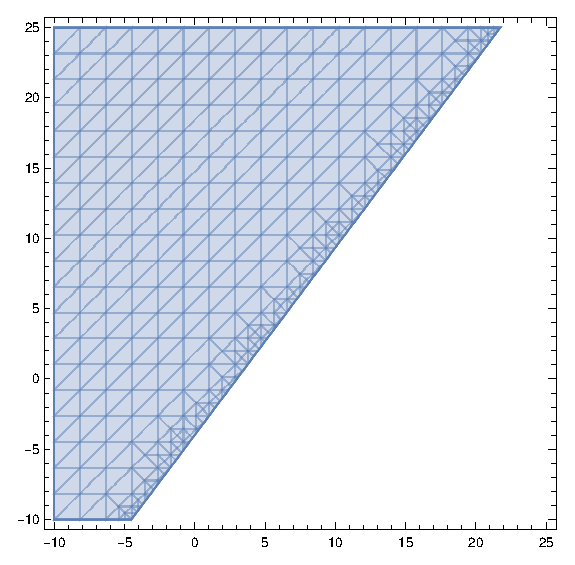
\includegraphics[width=0.99\textwidth]
    {inc/1.eps}
  
    \caption{Область $(4x-3y\leq 12)$}

    \label{fig:1}
  \end{minipage}
  \begin{minipage}{0.32\textwidth}
    \centering

    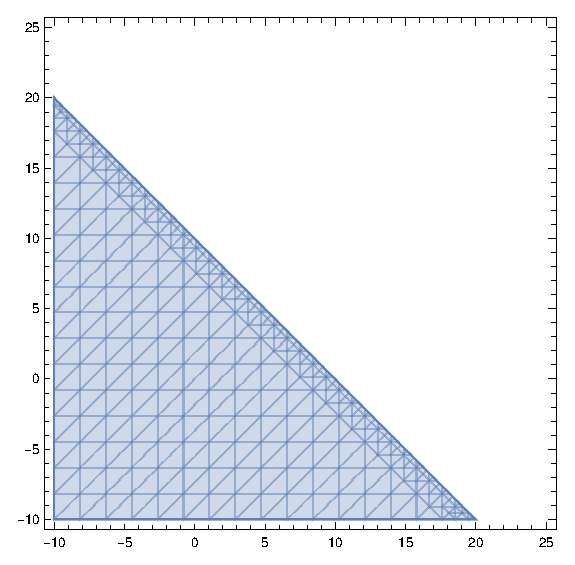
\includegraphics[width=0.99\textwidth]
    {inc/2.eps}
  
    \caption{Область $(x+y\leq 10)$}

    \label{fig:2}
  \end{minipage}
  \begin{minipage}{0.32\textwidth}
    \centering

    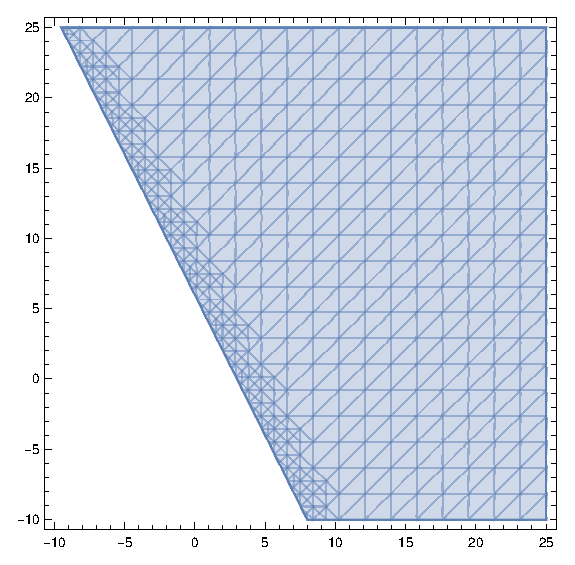
\includegraphics[width=0.99\textwidth]
    {inc/3.eps}
  
    \caption{Область $(2x+y\geq 6)$}

    \label{fig:3}
  \end{minipage}
\end{figure}

\subparagraph{2}
Для удобства нарисуем новый график.
Раскрасим его цветами.
Учитывая, что существует условие не отрицательности переменной,
заштрихуем получившуюся область.

Теперь в этой области нужно найти точку,
в которой функция $\mathbb{Z}$ принимает максимальное и минимальное значение.

$\mathbb{Z} =-2x+2x \to \text{max, min}$

Если мы запишем градиент функции, то это будет вектор, координатами которого будет частные производные функции.

$\text{grad }\mathbb{Z} = \{-2; 2\} = \bar{c}$

Он называется условным вектором и показывает направление максимального роста функции.

Общий график смотри на рисунке~\ref{fig:456}.

\begin{figure}[!htb]\centering
  \begin{minipage}{0.32\textwidth}
    \centering

    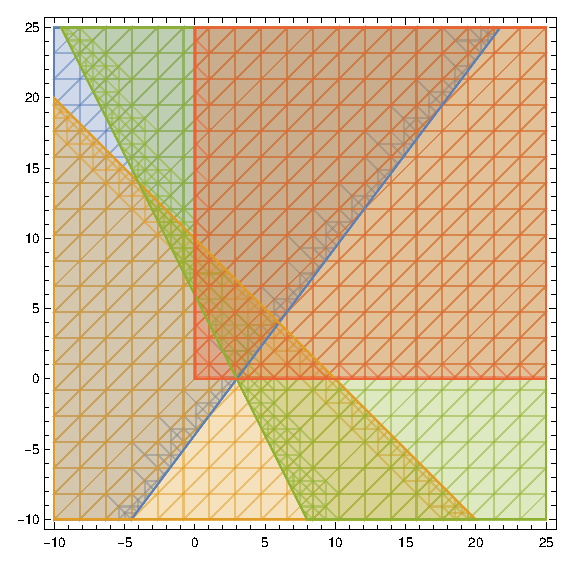
\includegraphics[width=0.99\textwidth]
    {inc/4.eps}
  \end{minipage}
  \begin{minipage}{0.32\textwidth}
    \centering

    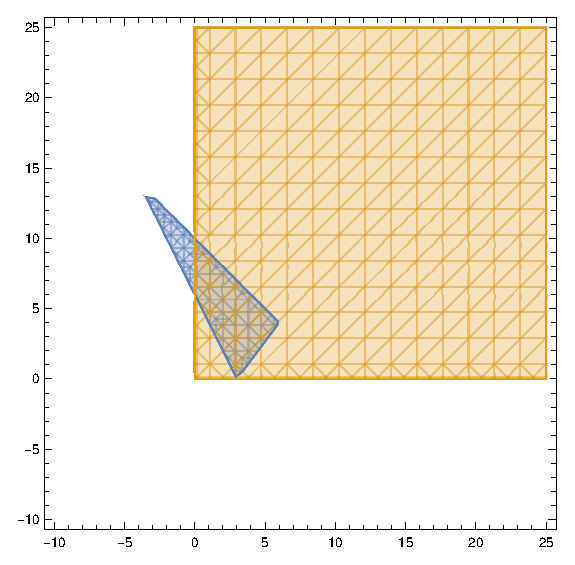
\includegraphics[width=0.99\textwidth]
    {inc/5.eps}
  \end{minipage}
  \begin{minipage}{0.32\textwidth}
    \centering

    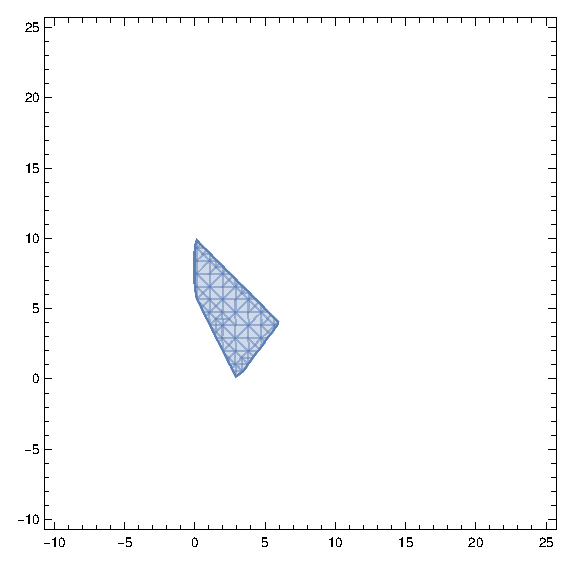
\includegraphics[width=0.99\textwidth]
    {inc/6.eps}
  \end{minipage}
  \caption{Общий график}
  \label{fig:456}
\end{figure}

Начертим этот вектор на графике. Теперь проведем вектору $\bar{c}$ перпендикуляр
и будем параллельно двигать в сторону вектора $\bar{c}$,
направления роста функции,
пока он не достигнет крайнего значения области.

И так мы дошли до крайнего значения области (-3; 0) - для max и (0; 10) - для min.

Значит в точке (3;0) - функция достигает максимума,
в точке (0;10) - функция достигает минимума.

$\mathbb{Z}_{max}$ - это значение в точке (3; 0).

$\mathbb{Z}_{min}$ - это значение в точке (0; 10).

$\mathbb{Z}_{max} = \mathbb{Z}(3; 0) = -2\cdot 3 + 2\cdot 0 = -6$

$\mathbb{Z}_{min} = \mathbb{Z}(0; 10) = -2\cdot 0 + 2 \cdot 10 = 20$

\subparagraph{} \textbf{Ответ}: $\mathbb{Z}_{max} = \mathbb{Z}(3;0)=-6$, $\mathbb{Z}_{min} = \mathbb{Z}(0; 10) = 20$.

\newpage

\begin{center}
\textbf{Проверка max через WinQSB}
\end{center}

На VirtualBox \cite{VirtualBox} устанавливаем WinXP \cite{WinXP}, а на неё программу WinSQB \cite{WinSQB}.

Пуск > WinQSB > Linear and Integer Programming > File > New Problem

Problem Title: MO\_PO4\_190333\_00\_max

Number of Variables: 2

Number of Constraints: 3

Object Criterion > Maxamization

OK> Заполняем таблицу

\begin{table}[h!]
  \centering
  \begin{tabular}{ |l||c|c|c|c| } 
    \hline
    Variable & X1 & X2 & Direction & R. H. S \\ \hline
    \hline
    Maximaze & -2 & 2 &  & \\ \hline
    C1 & 4 & -3 & <= & 12 \\ \hline
    C2 & 1 & 1 & <= & 10 \\ \hline
    C3 & 2 & 1 & >= & 6 \\ \hline
    LowerBound & 0 & 0 &  & \\ \hline
    UpperBound & M & M &  & \\ \hline
    VariableType & Continious & Continious &  & \\ \hline
  \end{tabular}
\end{table}

Жмем розовую кнопку > ОК

Options > Change XY Ranges and Colors > Background (жмем, пока не получим белый цвет) > ОК

Options > Change XY Variables > OK

File > Save As > 1.bmp. Результат на рисунке~\ref{fig:max}.

\begin{figure}[!htb]
  \centering

  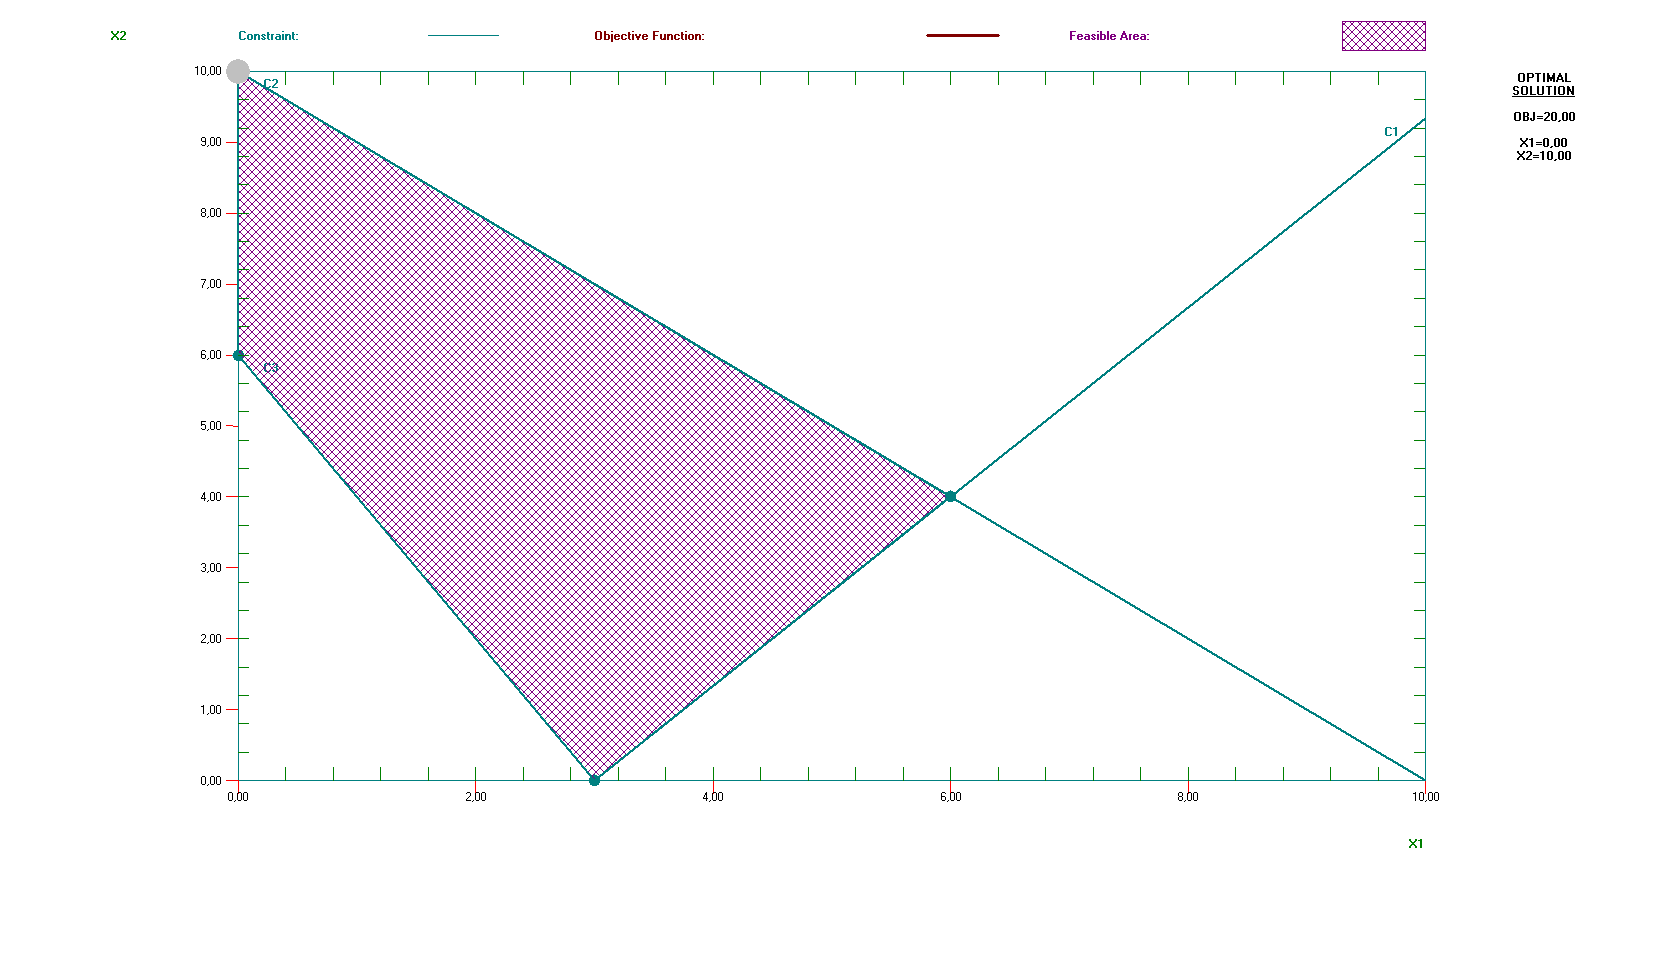
\includegraphics[width=16cm]
  {inc/max.png}

  \caption{Ищем max через WinSQB}
  \label{fig:max}
\end{figure}

\textbf{Вывод}: Получили в программе 20. Ручным способом получили 20. Результаты равны, значит решили верно.

\newpage

\begin{center}
\textbf{Проверка min через WinQSB}
\end{center}

На VirtualBox \cite{VirtualBox} устанавливаем WinXP \cite{WinXP}, а на неё программу WinSQB \cite{WinQSB}.

Пуск > WinQSB > Linear and Integer Programming > File > New Problem

Problem Title: MO.PO4.190333-00\_min

Number of Variables: 2

Number of Constraints: 3

Object Criterion > Minimization

OK> Заполняем таблицу

\begin{table}[h!]
  \centering
  \begin{tabular}{ |l||c|c|c|c| } 
    \hline
    Variable & X1 & X2 & Direction & R. H. S \\ \hline
    \hline
    Minimize & -2 & 2 &  & \\ \hline
    C1 & 4 & -3 & <= & 12 \\ \hline
    C2 & 1 & 1 & <= & 10 \\ \hline
    C3 & 2 & 1 & >= & 6 \\ \hline
    LowerBound & 0 & 0 &  & \\ \hline
    UpperBound & M & M &  & \\ \hline
    VariableType & Continious & Continious &  & \\ \hline
  \end{tabular}
\end{table}

Жмем розовую кнопку > ОК

Options > Change XY Ranges and Colors > Background (жмем, пока не получим белый цвет) > ОК

Options > Change XY Variables > OK

File > Save As > 1.bmp. Результат на рисунке~\ref{fig:min}.

\begin{figure}[!htb]
  \centering

  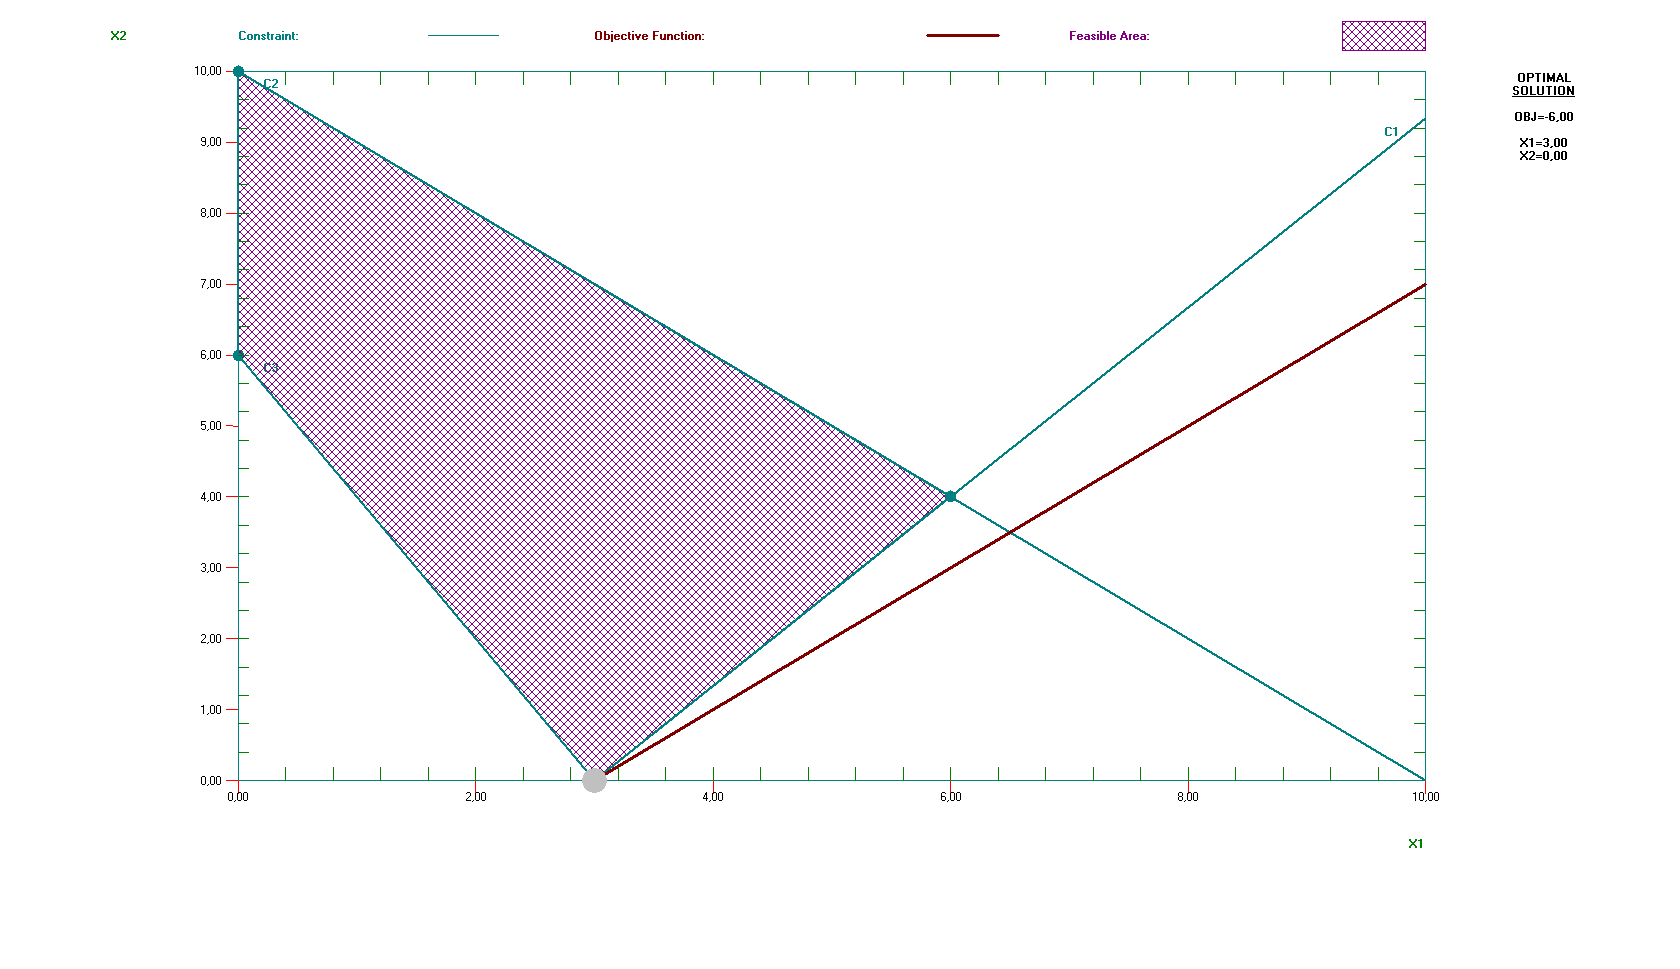
\includegraphics[width=16cm]
  {inc/min.png}

  \caption{Ищем min через WinSQB}
  \label{fig:min}
\end{figure}

\textbf{Вывод}: Получили в программе -6. Ручным способом получили -6. Результаты равны, значит решили верно.
